\documentclass[]{beamer}
\usepackage{lmodern}

\usetheme{CambridgeUS} % try Madrid, Pittsburgh
\usecolortheme{beaver}
\usefonttheme[onlymath]{serif} % try "professionalfonts"

\setbeamertemplate{itemize items}[default]
\setbeamertemplate{enumerate items}[default]

\usepackage{amsmath, amsfonts, latexsym, mathtools, extarrows}
\DeclareMathOperator*{\argmin}{arg\,min}
\DeclareMathOperator*{\argmax}{arg\,max}

\usepackage{pifont}
\usepackage{hyperref}
\usepackage{comment}

\usepackage[normalem]{ulem}
\newcommand{\middlewave}[1]{\raisebox{0.5em}{\uwave{\hspace{#1}}}}

\usepackage{graphicx, subcaption}

\usepackage{algorithm}
\usepackage[noend]{algpseudocode}

\newcommand{\pno}[1]{\textcolor{blue}{\scriptsize [Problem: #1]}}
\newcommand{\set}[1]{\{#1\}}

\newcommand{\cmark}{\textcolor{red}{\ding{51}}}
\newcommand{\xmark}{\textcolor{red}{\ding{55}}}
%%%%%%%%%%%%%%%%%%%%%%%%%%%%%%%%%%%%%%%%%%%%%%%%%%%%%%%%%%%%%%
% for fig without caption: #1: width/size; #2: fig file
\newcommand{\fignocaption}[2]{
  \begin{figure}[htp]
    \centering
      \includegraphics[#1]{#2}
  \end{figure}
}

% for fig with caption: #1: width/size; #2: fig file; #3: fig caption
\newcommand{\fig}[3]{
  \begin{figure}[htp]
    \centering
      \includegraphics[#1]{#2}
      \caption[labelInTOC]{#3}
  \end{figure}
}

\newcommand{\titletext}{Decompositions of Graphs}

\newcommand{\tx}{%
  \section*{}
  \begin{frame}[noframenumbering]
	\fignocaption{width = 0.50\textwidth}{figs/thankyou.jpg}
  \end{frame}
}
%%%%%%%%%%%%%%%%%%%%
\title[\titletext]{\titletext}
\subtitle{}

\author[Hengfeng Wei]{Hengfeng Wei}
\titlegraphic{
\includegraphics[height = 1.5cm]{figs/qrcode-alg-ta-20170524.png}}
\institute{hfwei@nju.edu.cn}
\date{May 20, 2017 -- May 24, 2017}

\AtBeginSection[]{
  \begin{frame}[noframenumbering, plain]
    \frametitle{\titletext}
    \tableofcontents[currentsection, sectionstyle=show/shaded, subsectionstyle=show/show/hide]
  \end{frame}
}

%%%%%%%%%%
\begin{document}
\maketitle

\section{DFS and BFS}

%%%%%%%%%%%%%%%%%%%%
\begin{frame}{Turing Award}
  \begin{columns}
	\column{0.50\textwidth}
	  \fignocaption{width = 0.40\textwidth}{figs/hopcroft.jpg}{\centerline{John Hopcroft}}
	\column{0.50\textwidth}
	  \fignocaption{width = 0.35\textwidth}{figs/tarjan.png}{\centerline{Robert Tarjan}}
  \end{columns}

  \vspace{0.50cm}
  \begin{quote}
	``For fundamental achievements in the design and analysis of algorithms and data structures.'' \\
	\hfill --- Turing Award, 1986
  \end{quote}
\end{frame}
%%%%%%%%%%%%%%%%%%%%
\begin{frame}{Depth-first search}
  \fignocaption{width = 0.55\textwidth}{figs/dfs-paper-tarjan}

  \uncover<2->{
	\begin{quote}
	  {\small ``We \textcolor{red}{have seen} how the depth-first search method may be used in the construction of
	  very efficient graph algorithms. $\dots$ \\
	  Depth-first search \textcolor{red}{is} a powerful technique with many applications.''}
	\end{quote}
  }

  \begin{alertblock}{Reference}
	\begin{itemize}
	  \item ``Depth-First Search And Linear Graph Algorithms'' by Robert Tarjan.
	\end{itemize}
  \end{alertblock}
\end{frame}
%%%%%%%%%%%%%%%%%%%%
\begin{frame}{Graph decomposition}
  \begin{center}
	Graph decomposition vs. Graph traversal \\[10pt]
	Structures!
  \end{center}

  \pause
  \begin{enumerate}
	\item states of vertices
	\item types of edges
	\item lifetime of vertices (DFS)
	  \begin{itemize}
	    \item $v: \text{d}[v], \text{f}[v]$
	    \item $\text{f}[v]$: DAG, SCC
	    \item $\text{d}[v]$: biconnectivity
	  \end{itemize}
  \end{enumerate}
\end{frame}
%%%%%%%%%%%%%%%%%%%%
\begin{frame}{Types of edges}
  \begin{definition}[Classifying edges]
    Given a DFS/BFS traversal $\Rightarrow$ DFS/BFS tree:
	\begin{description}[Forward edge:]
	  \item[Tree edge:] $\to$ child
	  \item[Back edge:] $\to$ ancestor
	  \item[Forward edge:] $\to$ \emph{nonchild} descendant
	  \item[Cross edge:] $\to$ neither ancestor nor descendant
    \end{description}
  \end{definition}

  \pause
  \begin{alertblock}{Remarks}
    \begin{itemize}
      \item applicable to both DFS and BFS
      \item w.r.t. DFS/BFS trees
    \end{itemize}
  \end{alertblock}
\end{frame}
%%%%%%%%%%%%%%%%%%%%
\begin{frame}{Types of edges (Problem 5.18)}
  \begin{figure}
	\begin{subfigure}{0.50\linewidth}
	  \centering
	  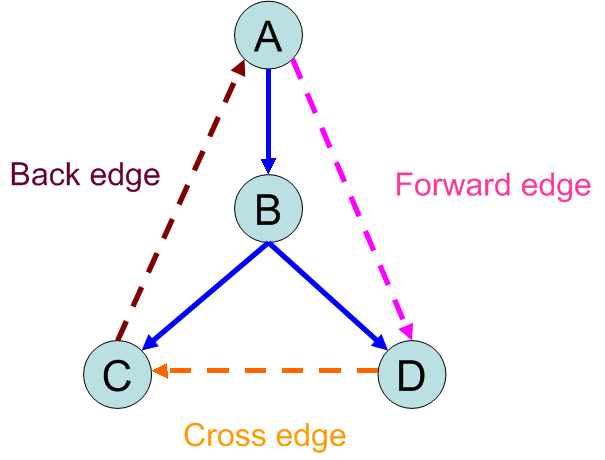
\includegraphics[width=0.50\textwidth]{figs/dfs-digraph.png}
	  \caption{DFS on directed graph.}
	\end{subfigure}%
	\begin{subfigure}{0.50\linewidth}
	  \centering
	  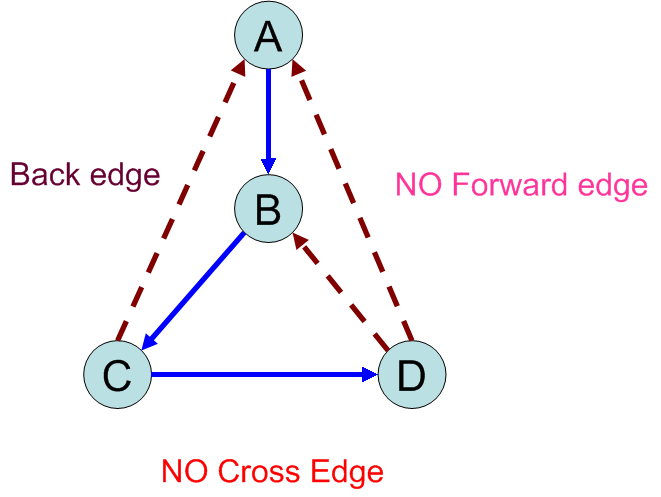
\includegraphics[width=0.50\textwidth]{figs/dfs-undirected.png}
	  \caption{DFS on undirected graph.}
	\end{subfigure}

	\begin{subfigure}{0.50\linewidth}
	  \centering
	  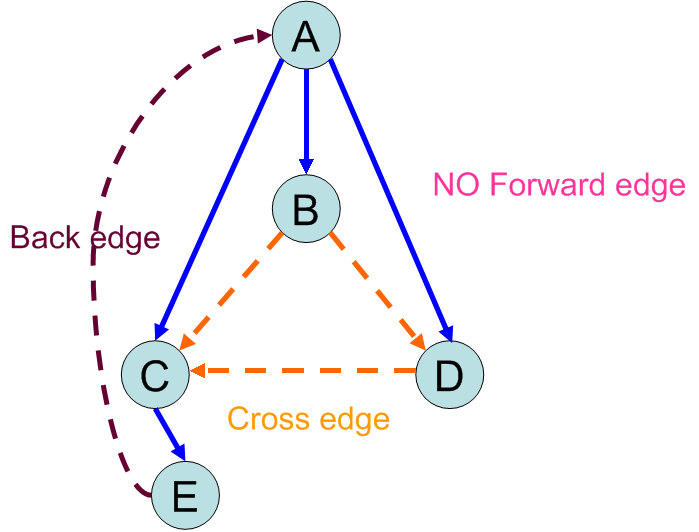
\includegraphics[width=0.50\textwidth]{figs/bfs-digraph.png}
	  \caption{BFS on directed graph.}
	\end{subfigure}%
	\begin{subfigure}{0.50\linewidth}
	  \centering
	  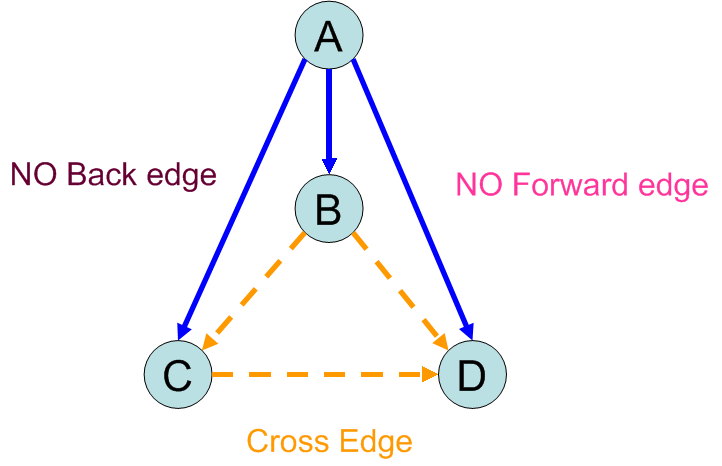
\includegraphics[width=0.60\textwidth]{figs/bfs-undirected.png}
	  \caption{BFS on undirected graph.}
	\end{subfigure}
  \end{figure}
\end{frame}
%%%%%%%%%%%%%%%%%%%%
\begin{frame}{Types of edges}
  \begin{exampleblock}{DFS tree and BFS tree coincide (Additional)}
    $G = (V,E), v \in V$. \\
	DFS tree $T$ = BFS tree $T'$.

    \begin{itemize}
      \item $G$ is an undirected graph $\implies G = T$
      \item $G$ is a digraph $\xLongrightarrow{?} G = T$
    \end{itemize}
  \end{exampleblock}

  \pause
  \begin{itemize}
	\item $T$: tree + back \emph{vs.} $T'$: tree + cross
	\pause
	\item $T$: tree + back + forward + cross \emph{vs.} $T'$: tree + back + cross 
  \end{itemize}
\end{frame}
%%%%%%%%%%%%%%%%%%%%
\begin{frame}{Lifttime of vertices in DFS}
  \begin{theorem}[Disjoint or contained]
	\begin{gather*}
	  \forall u,v: \\
	  [_{u} \; ]_{u} \cap [_{v} \; ]_{v} = \emptyset \\
	  \bigvee \\
	  ([_{u} \; ]_{u} \subsetneqq [_{v} \; ]_{v} \lor [_{v} \; ]_{v} \subsetneqq [_{u} \; ]_{u})
	\end{gather*}
  \end{theorem}

  \pause

  \begin{proof}
	\fignocaption{width = 0.30\textwidth}{figs/stack.png}
  \end{proof}
\end{frame}
%%%%%%%%%%%%%%%%%%%%
\begin{frame}{Ancestor/descendant relation}
  \begin{exampleblock}{Preprocessing for ancestor/descendant relation (Problem 5.23)}
    \begin{itemize}
      \item binary tree $T = (V, E)$ (tree)
      \item $r \in V$
    \end{itemize}
  \end{exampleblock}

  \[
	v: \text{d}[v], \text{f}[v]
  \]

  \pause
  \begin{alertblock}{Question}
    $\forall v$: how many descendants?

	\pause
    \[
	  (\text{f}[v] - \text{d}[v] - 1) / 2
	\]
  \end{alertblock}
\end{frame}
%%%%%%%%%%%%%%%%%%%%
\begin{frame}{Edge types and lifetime of vertices in DFS}
  \begin{exampleblock}{Edge types and lifetime of vertices in DFS (Problem 5.2)}
    $\forall u \to v$:
    \begin{itemize}
      \item tree/forward edge: $[_{u}\; [_{v}\; ]_{v}\; ]_{u}$
      \item back edge: $[_{v}\; [_{u}\; ]_{u}\; ]_{v}$
      \item cross edge: $[_{v}\; ]_{v}\; [_{u}\; ]_{u}$
    \end{itemize}
  \end{exampleblock}

  \pause

  \begin{alertblock}{Remark}
    \begin{itemize}
      \item $\text{f}[v] < \text{d}[u]$: cross edge
      \item $\text{f}[u] < \text{f}[v]$: back edge
		\pause
		\[
		  u \to v \iff \text{f}[v] < \text{f}[u]
		\]
    \end{itemize}
  \end{alertblock}
\end{frame}
%%%%%%%%%%%%%%%%%%%%
\begin{frame}{Height and diameter of tree}
  \begin{exampleblock}{Height and diameter of tree (Problem 5.21)}
	Binary tree $T = (V, E)$ with $|V| = n$:
	\begin{itemize}
	  \item height ($O(n)$)
	  \item diameter ($O(n)$)
	\end{itemize}
  \end{exampleblock}

  \begin{alertblock}{Question}
	Diameter of a tree \emph{without} designated root?
  \end{alertblock}
\end{frame}
%%%%%%%%%%%%%%%%%%%%
\begin{frame}{Perfect subtree}
  \begin{exampleblock}{Perfect subtree (Problem 5.22)}
	\begin{itemize}
	  \item binary tree $T = (V, E)$
	  \item root $r \in V$
	  \item goal: find all perfect subtrees
	\end{itemize}
  \end{exampleblock}
\end{frame}
%%%%%%%%%%%%%%%%%%%%
\begin{frame}{Counting shortest paths}
  \begin{exampleblock}{Counting shortest paths (Problem 5.26)}
  \end{exampleblock}
\end{frame}
%%%%%%%%%%%%%%%%%%%%

\section{Cycles}

%%%%%%%%%%%%%%%%%%%%
\begin{frame}{Cycle detection}
  \begin{exampleblock}{Cycle detection (Problem 5.24)}
	\begin{table}[ht]
	  \centering
	  \renewcommand{\arraystretch}{1.1}
	  \begin{tabular}{c||c|c}
	    \hline
		& Digraph 			& Undirected graph  \\ \hline \hline
		DFS & {\uncover<2->{back edge $\iff$ cycle}}
		& {\uncover<3->{back edge $\iff$ cycle}}
		\\ \hline
		BFS & {\uncover<5->{\begin{tabular}[c]{@{}l@{}}back edge $\implies$ cycle\\ cycle \textcolor{red}{$\centernot\implies$} back edge \end{tabular}}}
		& {\uncover<4->{cross edge $\iff$ cycle}}
		\\ \hline
	  \end{tabular}
	\end{table}
  \end{exampleblock}

  \begin{columns}
	\column{0.50\textwidth}
	  \uncover<6->{\fignocaption{width = 0.30\textwidth}{figs/bfs-digraph-cycle-without-back.png}}
	\column{0.50\textwidth}
	  \uncover<7->{%
		\begin{alertblock}{Remark}
		  How to identify back edges?
		\end{alertblock}}
  \end{columns}
\end{frame}
%%%%%%%%%%%%%%%%%%%%
\begin{frame}{Edge deletion}
  \begin{exampleblock}{Edge deletion (Problem 5.20)}
    \begin{itemize}
      \item connected, undirected graph $G$
      \item $\exists? e \in E: G \setminus e$ is connected?
      \item $O(|V|)$
    \end{itemize}
  \end{exampleblock}

  \pause
  \[
	\exists \text{ cycle} \iff \exists \text{ such } e
  \]

  \pause
  \[
	\text{tree: } |E| = |V| - 1 \implies \text{ check } |E| \ge |V|
  \]
\end{frame}
%%%%%%%%%%%%%%%%%%%%
\begin{frame}{Orientation of undirected graph}
  \begin{exampleblock}{Orientation of undirected graph (Problem 5.9)}
	\begin{itemize}
      \item undirected (connected) graph $G$ 
	  \item edges oriented \emph{s.t.} 
		\[
		  \forall v, \text{in}[v] \ge 1
		\]
	\end{itemize}
  \end{exampleblock}

  \pause
  \[
	\text{orientation} \iff \exists \text{ cycle } C
  \]

  \pause
  \[
	\text{BFS/DFS from } v \in C
  \]
\end{frame}
%%%%%%%%%%%%%%%%%%%%
\begin{frame}{Shortest cycle of undirected graph}
  \begin{exampleblock}{Shortest cycle of undirected graph (Problem 5.8)}
	Shortest cycle of $G$:
	\begin{itemize}
	  \item DFS on $G$
	  \item $\forall v: \text{level}[v]$
	  \item back edge $u \to v: \text{level}[u] - \text{level}[v] + 1$
	\end{itemize}
  \end{exampleblock}

  \pause
  \begin{alertblock}{Question}
	What about digraphs?
  \end{alertblock}
\end{frame}
%%%%%%%%%%%%%%%%%%%%

\section{DAG}

%%%%%%%%%%%%%%%%%%%%
\begin{frame}{DAG}
  \begin{center}
    no back edge $\iff$ DAG \pause $\iff$ $\exists$ topo. ordering
  \end{center}

  \begin{block}{Toposort algorithm by Tarjan (probably), 1976}
    DFS on digraph, $u \to v$:
    \begin{itemize}
	  \item \sout{back edge:} $\text{f}[u] < \text{f}[v]$
      \item others: $\text{f}[u] > \text{f}[v]$
    \end{itemize}

	\pause
    \[ 
	  u \to v \implies \text{f}[u] > \text{f}[v]
	\]

	\pause
    \begin{center}
	  Toposort: sort vertices in \textcolor{blue}{\emph{decreasing}} order of their \textcolor{blue}{\emph{finish}} times.
    \end{center}
  \end{block}
\end{frame}
%%%%%%%%%%%%%%%%%%%%
\begin{frame}{Kahn's toposort algorithm}
  \begin{exampleblock}{Kahn's toposort algorithm (1962; Problem 5.11) }
    \begin{itemize}
      \item queue for source vertices ($\text{in}[v] = 0$)
      \item repeat: dequeue $v$, delete it, output it
    \end{itemize}
  \end{exampleblock}

  \pause
  \begin{lemma}
	Every DAG has at least one source (and at least one sink vertex).
  \end{lemma}

  \pause
  \begin{alertblock}{Question}
	What if $G$ is not a DAG?
  \end{alertblock}
\end{frame}
%%%%%%%%%%%%%%%%%%%%
\begin{frame}{Taking courses}
  \begin{exampleblock}{Taking courses in few semesters (Problem 5.14)}
	\begin{itemize}
	  \item $n$ courses
	  \item $c_1 \to c_2$
	  \item goal: taking courses in few semesters
	\end{itemize}
  \end{exampleblock}

  \pause
  \begin{center}
	critical path \emph{OR} longest path
  \end{center}

  \pause
  \begin{alertblock}{Remark}
	For general digraph, LONGEST-PATH is NP-hard.
  \end{alertblock}
\end{frame}
%%%%%%%%%%%%%%%%%%%%
\begin{frame}{Line up}
  \begin{exampleblock}{Line up (Problem 5.16)}
    \begin{enumerate}
      \item $i$ hates $j$: $i \prec j$
      \item $i$ hates $j$: $\# i < \# j$
    \end{enumerate}
  \end{exampleblock}
\end{frame}
%%%%%%%%%%%%%%%%%%%%
\begin{frame}{Hamiltonian path in DAG}
  \begin{exampleblock}{Hamiltonian path in DAG (Problem 5.10)}
    \begin{itemize}
      \item DAG $G$
      \item HP: path visiting each vertex once
    \end{itemize}
  \end{exampleblock}

  \pause
  \begin{alertblock}{Remark}
    For general (di)graph, HP is NP-hard.
  \end{alertblock}

  \pause
  \[
	\text{DAG: } \exists \text{ HP} \iff \exists! \text{ topo. ordering}
  \]

  \begin{columns}
	\column{0.50\textwidth}
	  \pause
	  \begin{proof}
		$\Longleftarrow$: By contradiction. 
	  \end{proof}
	\column{0.50\textwidth}
	  \pause
	  Algorithms:
	  \begin{enumerate}
		\item toposort, check edges
		\item the Kahn toposort algorithm
	  \end{enumerate}
	\end{columns}
\end{frame}
%%%%%%%%%%%%%%%%%%%%

% file: sections/scc.tex

%%%%%%%%%%%%%%%%%%%%
\begin{frame}{}
  \begin{theorem}[Digraph as DAG (Problem $4.6$)]
    Every digraph is a dag of its SCCs.
  \end{theorem}

  \pause
  \vspace{0.60cm}
  \begin{center}
    \red{\large Two tiered structure of digraphs:} \\[10pt] 

    digraph $\equiv$ a \teal{dag} of SCCs \\[6pt]

    SCC: equivalence class over \teal{reachability}
  \end{center}
\end{frame}
%%%%%%%%%%%%%%%%%%%%
\begin{frame}{}
  \centerline{\red{\fbox{\large \text{digraph} $\equiv$ a \teal{dag} of SCCs}}}

  \vspace{0.50cm}
  \begin{exampleblock}{Kosaraju's SCC algorithm, $1978$}
    \begin{quote}
      \begin{center}
	{\large ``SCCs can be topo-sorted \\[3pt] in \red{decreasing} order of their highest \red{finish} time.''}
      \end{center}
    \end{quote}

    \pause
    \centerline{The vertice with the \red{highest} finish time is in a \red{source} SCC.}
  \end{exampleblock}

  \pause
  \vspace{0.60cm}
  \begin{enumerate}[(I)]
    \centering
  \item DFS on $G$; \; DFS/BFS on $G^{T}$ \\[8pt]
      \pause
    \item DFS on $G^{T}$;\; DFS/BFS on $G$
  \end{enumerate}
\end{frame}
%%%%%%%%%%%%%%%%%%%%
\begin{frame}{}
  \begin{exampleblock}{Kosaraju's SCC algorithm, $1978$ (Problem $4.7$)}
    \begin{center}
      $1$st DFS $\xLongrightarrow{?}$ BFS \\[8pt]
      $2$nd DFS $\xLongrightarrow{?}$ BFS
    \end{center}
  \end{exampleblock}

  \pause
  \vspace{0.50cm}
  \begin{description}
    \centering
    \item[$1$st DFS:] \brown{toposort} between SCCs
    \item[$2$nd DFS:] \brown{reachability} within an SCC
  \end{description}

  \pause
  \vspace{0.50cm}
  \centerline{\red{\fbox{\large digraph $\equiv$ a \teal{dag} of SCCs}}}
\end{frame}
%%%%%%%%%%%%%%%%%%%%
\begin{frame}{}
  \begin{exampleblock}{One-to-all reachability in a digraph (Problem 5.12)}
    \[
      v: v \leadsto^{?} \forall u
    \]
    \[
      \red{\exists?\; v: v \leadsto \forall u}
    \]
  \end{exampleblock}

  \pause
  \vspace{0.60cm}
  \centerline{\red{SCC}}

  \[
    \exists!\; \text{source vertex } v \iff v \leadsto \forall u
  \]

  \pause
  \[
    \impliedby: \red{\exists!}\; \blue{\text{source}}
  \]

  \pause
  \centerline{$\implies$: By contradiction.}
  \[
    \exists u: v \not\leadsto u \land \text{in}[u] > 0 \implies \exists \text{ cycle}
  \]
\end{frame}
%%%%%%%%%%%%%%%%%%%%
\begin{frame}{}
  \begin{exampleblock}{Impacts of vertices in a digraph (Problem $4.18$)}
    \[
      \text{impact}(v) = |\set{w \neq v: v \leadsto w}|
    \]

    \begin{itemize}
      \centering
      \item $\argmin_{v} \text{impact}(v)$
      \item $\argmax_{v} \text{impact}(v)$
    \end{itemize}
  \end{exampleblock}

  \pause
  \[
    \argmin_{v} \text{impact}(v) \in \text{\teal{sink} SCC of smallest cardinality}
  \]
  \pause
  \[
    \argmax_{v} \text{impact}(v) \in \text{\teal{source} SCC}
  \]

  \pause
  \vspace{0.30cm}
  \centerline{\red{$Q:$ $\forall v,$ computing $\text{impact}(v)$}}
\end{frame}
%%%%%%%%%%%%%%%%%%%%
\begin{frame}<presentation:0>[noframenumbering]
  \begin{exampleblock}{One-way streets (Problem $4.21$)}
	Digraph $G$ for city:
    \begin{enumerate}
      \item $\forall u,v: u \leftrightsquigarrow v$
      \item $s: s \leadsto v \leadsto s$
    \end{enumerate}
  \end{exampleblock}

  \pause
  \[
	(2)\; \set{v \mid s \leadsto v} \text{ is an SCC}
  \]
\end{frame}
%%%%%%%%%%%%%%%%%%%%
\begin{frame}<presentation:0>[noframenumbering]
  \begin{exampleblock}{Connectivity (Problem $4.11$)}
	\begin{description}[Example:]
	  \item[Prove:] connected undirected graph $G$: 
		\[
		  \exists v: G \setminus v \text{ is still connected}
		\]
	  \item[Example:] strongly connected digraph $G$:
		\[
		  \exists v: G \setminus v \text{ is not strongly connected}
		\]
	  \item[Example:] digraph $G$ with 2 SCCs:
		\[
		  (G + e) \text{ is not strongly connected}
		\]
	\end{description}
  \end{exampleblock}
\end{frame}
%%%%%%%%%%%%%%%%%%%%
\begin{frame}<presentation:0>[noframenumbering]
  \begin{exampleblock}{2SAT (Problem $4.23$)}
    \[
      I: (x_1 \lor \overline{x_2}) \land (\overline{x_1} \lor \overline{x_3}) \land (x_1 \lor x_2) \land (\overline{x_3} \lor x_4) \land (\overline{x_1} \lor x_4)
    \]
  \end{exampleblock}

  \pause
  \[
    \alpha \lor \beta \equiv \overline{\alpha} \to \beta \equiv \overline{\beta} \to \alpha
  \]

  \pause
  \begin{center}
    Implication graph $G_I$.
  \end{center}

  \pause
  \begin{theorem}[2SAT]
    \[
      \exists \text{ SCC } \exists x: v_x \in \text{SCC} \land v_{\overline{x}} \in \text{SCC} \iff I \text{ is not satisfiable}.
    \]
  \end{theorem}

  \pause
  \begin{alertblock}{Reference:}
    \begin{itemize}
      \item {\it ``A Linear-time Algorithm for Testing the Truth of Certain Quantified Boolean Formulas''} 
	by Bengt Aspvall, Michael Plass, and Robert Tarjan, $1979$.
    \end{itemize}
  \end{alertblock}
\end{frame}
%%%%%%%%%%%%%%%%%%%%
\begin{frame}<presentation:0>[noframenumbering]
  % \begin{gather*}
  %   (x_0\lor x_2)\land(x_0\lor\lnot x_3)\land(x_1\lor\lnot x_3)\land(x_1\lor\lnot x_4)\land\\
  %   (x_2\lor\lnot x_4)\land (x_0\lor\lnot x_5)\land (x_1\lor\lnot x_5)\land (x_2\lor\lnot x_5)\land\\
  %   (x_3\lor x_6)\land (x_4\lor x_6)\land (x_5\lor x_6)
  % \end{gather*}
  \begin{columns}
    \column{0.50\textwidth}
      % \fignocaption{width = 0.80\textwidth}{figs/2sat-implication-graph-wiki.png}
      \fignocaption{width = 0.80\textwidth}{figs/2sat-implication-graph.pdf}
    \column{0.50\textwidth}
      \pause
      \fignocaption{width = 0.80\textwidth}{figs/2sat-implication-graph.png}
  \end{columns}
\end{frame}
%%%%%%%%%%%%%%%%%%%%
\begin{frame}<presentation:0>[noframenumbering]
  \begin{exampleblock}{Odd cycle in digraph (Additional Problem)}
    Find an odd cycle in a digraph $G$.
  \end{exampleblock}

  \pause
  \begin{lemma}
    A digraph $G$ has an odd directed cycle $\iff$ $\exists \text{scc}: $ scc is non-bipartite (when treated undirected).
  \end{lemma}

  \pause
  \begin{alertblock}{Question}
	To prove the lemma and design an algorithm.
  \end{alertblock}
  \begin{proof}
    $\Longleftarrow$: undirected $C$; oriented
      \begin{itemize}
    	\item odd directed cycle
    	\item choose a direction $\forall u \to v$: $\text{Len}(v \leadsto u)$ 
      \end{itemize}
  \end{proof}
\end{frame}
%%%%%%%%%%%%%%%%%%%%

% file: sections/biconn.tex

%%%%%%%%%%%%%%%%%%%%
\begin{frame}{}
  \centerline{\Large \textsc{Bicomp}: \red{\huge Back!}}

  \pause
  \begin{center}
    % file: sections/bicomp-dfs-tree.tex

\begin{tikzpicture} [level distance = 50pt, sibling distance = 20pt,
  edge from parent/.style= { % added code
      draw, edge from parent path = {(\tikzparentnode) -- (\tikzchildnode)}}]
  \tikzset{every tree node/.style = 
    {align = center, circle, draw, fill = blue!20, font = \Large, minimum size = 20pt}}
    \Tree [.\textcolor{red}{$r$}
	    [.\node (x) {$x$};
	       [.\node (ll) {};
	        \node (w) {\textcolor{red}{$w$}};
		$$
	       ]
	       [.\node (v) {\textcolor{red}{$v$}};
		 \node (u) {\textcolor{teal}{$u$}};
	       ]
            ]
	    [.$$ 
	      $$
	      $$
	    ] 
        ]

%     \path<+-> (u) edge[thick, teal, bend left] (x)
% 	(w) edge[thick, red, bend left = 45] (r)
% 	(v) edge[thick, red, bend right] (r);
	\uncover<3->{\draw[thick, teal, bend left] (u) to (x);}
	\uncover<4->{\draw[thick, red, bend left = 45] (w) to (r);}
	\uncover<5->{\draw[thick, red, bend right] (v) to (r);}
\end{tikzpicture}

  \end{center}
\end{frame}
%%%%%%%%%%%%%%%%%%%%

%%%%%%%%%%%%%%%%%%%%
\begin{frame}{}
  \centerline{\red{$\text{back}[v]$:} the earliest reachable ancestor of $v$} % by tree + back edges

  \vspace{0.30cm}
  \begin{enumerate}[(I)]
    \centering
    \item When and how to \brown{update} $\text{back}[v]$? \\[6pt]
    \item When and how to \brown{identify} a bicomponent?
  \end{enumerate}

  \pause
  \fignocaption{width = 0.30\textwidth}{figs/bicomp-dfs-alg}
\end{frame}
%%%%%%%%%%%%%%%%%%%%

%%%%%%%%%%%%%%%%%%%%
\begin{frame}{}
  \begin{exampleblock}{Initialization of $\text{back}[v]$ (Problem $4.9$)}
    \[
      \text{back}[v] = d[v] \text{\emph{ vs. }} \text{back}[v] = \infty \lor 2(n+1) 
    \]
  \end{exampleblock}

  \pause
  \vspace{0.30cm}
  \begin{description}[backtracking from $w$:]
    \item[tree edge ($\to v$):]   $\text{back}[v] = \red{d[v]}$
    \item[back edge ($v \to w$):] $\text{back}[v] = \min \set{\text{back}[v], d[w]}$
    \item[backtracking from $w$:] $\text{back}[v] = \min \set{\text{back}[v], \text{back}[w] = \teal{\text{wBack}}}$
  \end{description}

  \pause
  \begin{proof}
    \begin{columns}
      \column{0.30\textwidth}
	\centerline{if ever updated}
      \column{0.70\textwidth}
	\pause
	\centerline{if never updated:}
	\pause
	\[
	  \text{wBack} = \infty > d[v] \text{\emph{ vs. }} \pause \text{wBack} = d[w] > d[v]
	\]
    \end{columns}
    \vspace{-0.50cm}
  \end{proof}
\end{frame}
%%%%%%%%%%%%%%%%%%%%
\begin{frame}{}
  \begin{exampleblock}{Root cutnode $v$ (Problem $4.8$)}
    \[
      v \text{ is a cutnode} \iff \text{out}[v] \ge 2
    \]
  \end{exampleblock}

  \pause
  \fignocaption{width = 0.40\textwidth}{figs/cutnode-types.png}
\end{frame}
%%%%%%%%%%%%%%%%%%%%
\begin{frame}<presentation:0>[noframenumbering]
  \begin{exampleblock}{Planning a party (Problem $5.11$)}
	\begin{itemize}
	  \item undirected graph $G$
	  \item subgraph $G' = (V', E')$:
		\[
		  \forall v' \in V: K(v') \ge 5 \land D(v') \ge 5
		\]
	\end{itemize}
  \end{exampleblock}

  \pause
  \vspace{0.50cm}
  $K$-core of a graph:
  \[
    \forall v' \in V': \text{deg}[v'] \ge k
  \]

  \pause
  \vspace{0.50cm}
  \centerline{Iteratively delete nodes $v$ of $K(v) < 5 \lor D(v) < 5$}
\end{frame}
%%%%%%%%%%%%%%%%%%%%

\tx{}

\end{document}
%%%%%%%%%%
